\documentclass{article}

% Packages
\usepackage[a4paper, margin=1cm]{geometry}
\usepackage{graphicx}

\setlength\parindent{0pt}

\usepackage{textcomp}
\usepackage{gensymb}
\usepackage{amsmath}
\usepackage{amsfonts}

\usepackage{tikz}
\usepackage{pgfplots}
\pgfplotsset{compat=newest}
\usepackage{pgfplotstable}

\usepackage{subcaption}
\usepackage{graphicx}

\usepackage{physics}

\DeclareCaptionLabelSeparator{titik}{. }

\begin{document}
\captionsetup[figure]{labelfont={sc}, labelsep=titik}

\begin{center}
    \textbf{AE2202 Fluid Dynamics} \\
    \textbf{Homework 6}
\end{center}

\hfill

\textbf{Question 1}. A solid circular cylinder of radius $R$ rotates at angular velocity $\Omega$ in a viscous incompressible fluid that is at rest far from the cylinder, as in figure below. Make simplifying assumptions and derive the governing differential equation and boundary conditions for the velocity field $v_\theta$ in the fluid. What is the steady-state flow field for this problem?

\begin{figure}[h]
    \centering
    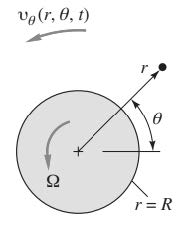
\includegraphics{Problem1.jpg}
    \caption{Illustration of Problem 1}
    \label{fig:figprob1}
\end{figure}

\textbf{\underline{Answer}}

Based on the description, the fluid surrounding the cylinder is viscous and incompressible and we only consider steady-sate condition. To simplify even further, we will assume (1) the fluid only move in the direction of $\theta$ and (2) uniform pressure distribution. We also have our boundary condition to be (1) the relative velocity of the fluid at the surface of the cylinder with respect the surfce is zero and (2) the velocity of the fluid far from the surface is zero.

We have our governing equation of Navier-Stokes Theorem:
\begin{equation}
    \rho \frac{d \mathbf{v}}{dt} = -\mathbf{\nabla}p + \mu \nabla^2 \mathbf{v} + \rho \mathbf{g}
\end{equation}
For cylindrical coordinates at $\theta$,
\begin{equation}
    \rho\left( \frac{\partial v_\theta}{\partial t} + v_r \frac{\partial v_\theta}{\partial r} + \frac{1}{r} v_\theta \frac{\partial v_\theta}{\partial \theta} + v_z \frac{\partial v_\theta}{\partial z} + \frac{v_r v_\theta}{r}\right) = -\frac{1}{r} \frac{\partial p}{\partial \theta} + \mu \left(\frac{1}{r} \frac{\partial}{\partial r}\left(r \frac{\partial v_\theta}{\partial r}\right) + \frac{1}{r^2} \frac{\partial^2 v_\theta}{\partial \theta^2} + \frac{\partial^2 v_\theta}{\partial z^2} + \frac{2}{r^2} \frac{\partial v_\theta}{\partial \theta} - \frac{v_\theta}{r^2}\right) + \rho g_\theta
\end{equation}
Applying our assumptions,
\begin{align*}
    0 + 0 + 0 + 0 + 0 &= 0 + \mu \left(\frac{1}{r} \frac{\partial}{\partial r}\left(r \frac{\partial v_\theta}{\partial r}\right) + 0 + 0 + 0 - \frac{v_\theta}{r^2}\right) + 0 \\
    \frac{1}{r} \frac{\partial}{\partial r}\left(r \frac{\partial v_\theta}{\partial r}\right) - \frac{v_\theta}{r^2} &= 0 \\
    \frac{\partial^2 v_\theta}{\partial r^2} + \frac{1}{r} \frac{\partial v_\theta}{\partial r} - \frac{v_\theta}{r^2} &= 0 \\
    v_\theta (r) &= c_1 r + \frac{c_2}{r} \left[\textrm{Euler-Cauchy Equation}\right]
\end{align*}
Rewriting our boundary conditions:
\begin{enumerate}
    \item $(v_\theta (R))_{\textrm{rel}} = 0 \Rightarrow (v_\theta (R)) = \Omega R$
    \item $\lim_{r \rightarrow \infty} (v_\theta (r)) = 0$
\end{enumerate}
For that BC 2. is valid, $c_1$ must be zero to ensure $v_\theta (r)$ not diverging to invinity when $r \rightarrow 0$. Thus,
\begin{align*}
    \Omega R &= \frac{c_2}{R} \\
    c_2 &= \Omega R^2
\end{align*}
Therefore, we got that
\begin{equation*}
    v_\theta (r) = \frac{\Omega R^2}{r}
\end{equation*}
    
\end{document}